\documentclass{report}
\usepackage[T1]{fontenc}
\usepackage{color}
\usepackage{amssymb}
\usepackage{pdfpages}
\usepackage{amsmath}
\usepackage{eurosym}
\usepackage{graphicx}
\usepackage{textcomp}
\usepackage{listings}
\usepackage{epigraph}
\usepackage{setspace}
\usepackage{array}
\usepackage{gensymb}
\usepackage{tikz}
\usepackage[some]{background}
\usepackage{geometry}
\usepackage[francais]{babel}


\begin{document}
\renewcommand{\contentsname}{Sommaire}
\renewcommand{\chaptername}{Partie}
\renewcommand{\thechapter}{\Roman{chapter}}

%\usepackage{lmodern}
%\usepackage{xspace}
%\usepackage{hyperref}

\definecolor{sup_strip_color}{rgb}{0.70,0.70,0.70}
\definecolor{inf_strip_color}{rgb}{0.00,0.00,0.00}

\DeclareFixedFont{\bigsf}{T1}{phv}{b}{n}{0.7cm}

\makeatletter                       
\def\printauthor{%                  
    {{\large \@author}}}              
\makeatother

\author{Zohour \textsc{Abouakil} ~\\ Sofia \textsc{Boutahar} ~\\ David \textsc{Courtinot} ~\\ Xiaowen \textsc{Ji} ~\\ Fabien \textsc{Sauce}}

\begin{titlepage}

\newgeometry{left=1cm,right=4cm}
\begin{tikzpicture}[overlay,remember picture]
% the black stripe with the title
\node[
  fill=inf_strip_color,
  anchor=north west,
  text width=\paperwidth,
  text height=2cm,
  text depth=2cm,
  inner xsep=1cm,
  font=\color{white}\bigsf 
  ] 
<<<<<<< HEAD
 at ([yshift=-2.5cm]current page.north west) (blackrect) {Plan de d\'{e}veloppement};
=======
 at ([yshift=-2.5cm]current page.north west) (blackrect) {Development plan};
>>>>>>> 04eedbcacdb0fd2dc91e65ebf589ebe6d5f75aee
% the khaki stripe
\path[fill=sup_strip_color] 
  (blackrect.north west) rectangle ++(\paperwidth,2.5cm);
\end{tikzpicture}

\vspace*{4.5cm}

\noindent
\begin{minipage}{0.35\linewidth}
    \begin{flushright}
        \printauthor
    \end{flushright}
\end{minipage} \hspace{15pt}
%
\begin{minipage}{0.02\linewidth}
    \rule{1pt}{175pt}
\end{minipage} \hspace{-10pt}
%
\begin{minipage}{0.6\linewidth}
\vspace{5pt}
\newenvironment{test}{\begin{center}}{\end{center}}
\hspace{10pt}
\begin{minipage}{\linewidth} 
Recherche de motifs dans un code C++ \`{a} l'aide de la logique temporelle
\end{minipage}
\end{minipage}

\end{titlepage}
\restoregeometry
\tableofcontents
<<<<<<< HEAD
\chapter{Project description and objectives}
=======
\chapter{Project description and objectives test test}
>>>>>>> 04eedbcacdb0fd2dc91e65ebf589ebe6d5f75aee

\section{Surroundings of the project}

\paragraph{}
\hspace{4mm}\textnormal{Le projet long \`{a} l'ENSEEIHT
	Organisation du projet}

\paragraph{}
\hspace{4mm}\textnormal{Le client c est qui ?? Les noms, leurs fonctions, les motivations du projet}

\paragraph{}
\hspace{4mm}\textnormal{Nos motivations -- pas sur}

\section{Project description}

\subsection{Main idea}

\subsection{Related technologies}

\vspace{4mm}
\begin{itemize}
\item Coccinelle\vspace{1mm}
\item Clang\vspace{1mm}
\end{itemize}

\subsection{Project parts}

\vspace{4mm}
\begin{itemize}
\item Parser\vspace{1mm}
\item CTL\vspace{1mm}
\item Model checking\vspace{1mm}
\end{itemize}

\subsection{To conclude}

\section{Final project}

\subsection{Define priorities}

\subsection{Deliverable documents}

\chapter{Project organization}

\section{Role definition}

\subsubsection{Project manager}

\paragraph{}
\hspace{4mm}\textnormal{}

\subsubsection{Quality manager}

\paragraph{}
\hspace{4mm}\textnormal{}

\subsubsection{Test manager}

\paragraph{}
\hspace{4mm}\textnormal{}

\subsubsection{Test manager}

\paragraph{}
\hspace{4mm}\textnormal{}

\subsubsection{Configuration manager}

\paragraph{}
\hspace{4mm}\textnormal{}

\subsubsection{Documentation manager}

\paragraph{}
\hspace{4mm}\textnormal{}

\subsubsection{Chain development}

\begin{center}
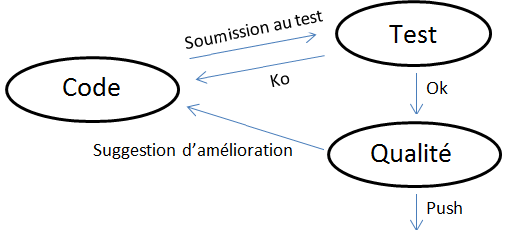
\includegraphics[scale=0.7]{data/cycle_qualite}
~\\~\\Figure II.1 - Sch\'{e}ma descriptif de la cha\^{i}ne de d\'{e}veloppement
\end{center}

<<<<<<< HEAD
\section{Development organisation}
=======
\section{Development organization}
>>>>>>> 04eedbcacdb0fd2dc91e65ebf589ebe6d5f75aee

\paragraph{}
\hspace{4mm}\textnormal{To secure our evolution we can use :}

<<<<<<< HEAD
\subsection{Use of Scrum method}

\paragraph{}
\hspace{4mm}\textnormal{We will try to use Scrum method, which is actually widely used, and 
recognised for its effectiveness. At first, we will define a 
\textit{product backlog} containing all desired functionalities in 
the final product. In fact, this report is also a part of \textit{product backlog}. Next, we will divide the project into 
three \textit{sprints} (which means iterations). A \textit{sprint backlog} is defined for each \textit{sprint}, including all we need 
to realise at the end of an iteration. Each \textit{sprint} lasts two weeks and lies in improve the software incrementally, so that it 
is close to \textit{product backlog}.}
=======
\subsection{Use of a software development framework : Scrum}

\paragraph{}
\hspace{4mm}\textnormal{}
>>>>>>> 04eedbcacdb0fd2dc91e65ebf589ebe6d5f75aee

\subsection{Team repartition approach}

\paragraph{}
\hspace{4mm}\textnormal{}

<<<<<<< HEAD
\section{Tasks organisation}
=======
\section{Tasks organization}
>>>>>>> 04eedbcacdb0fd2dc91e65ebf589ebe6d5f75aee

\subsection{Tasks definition}

\subsection{Planning}

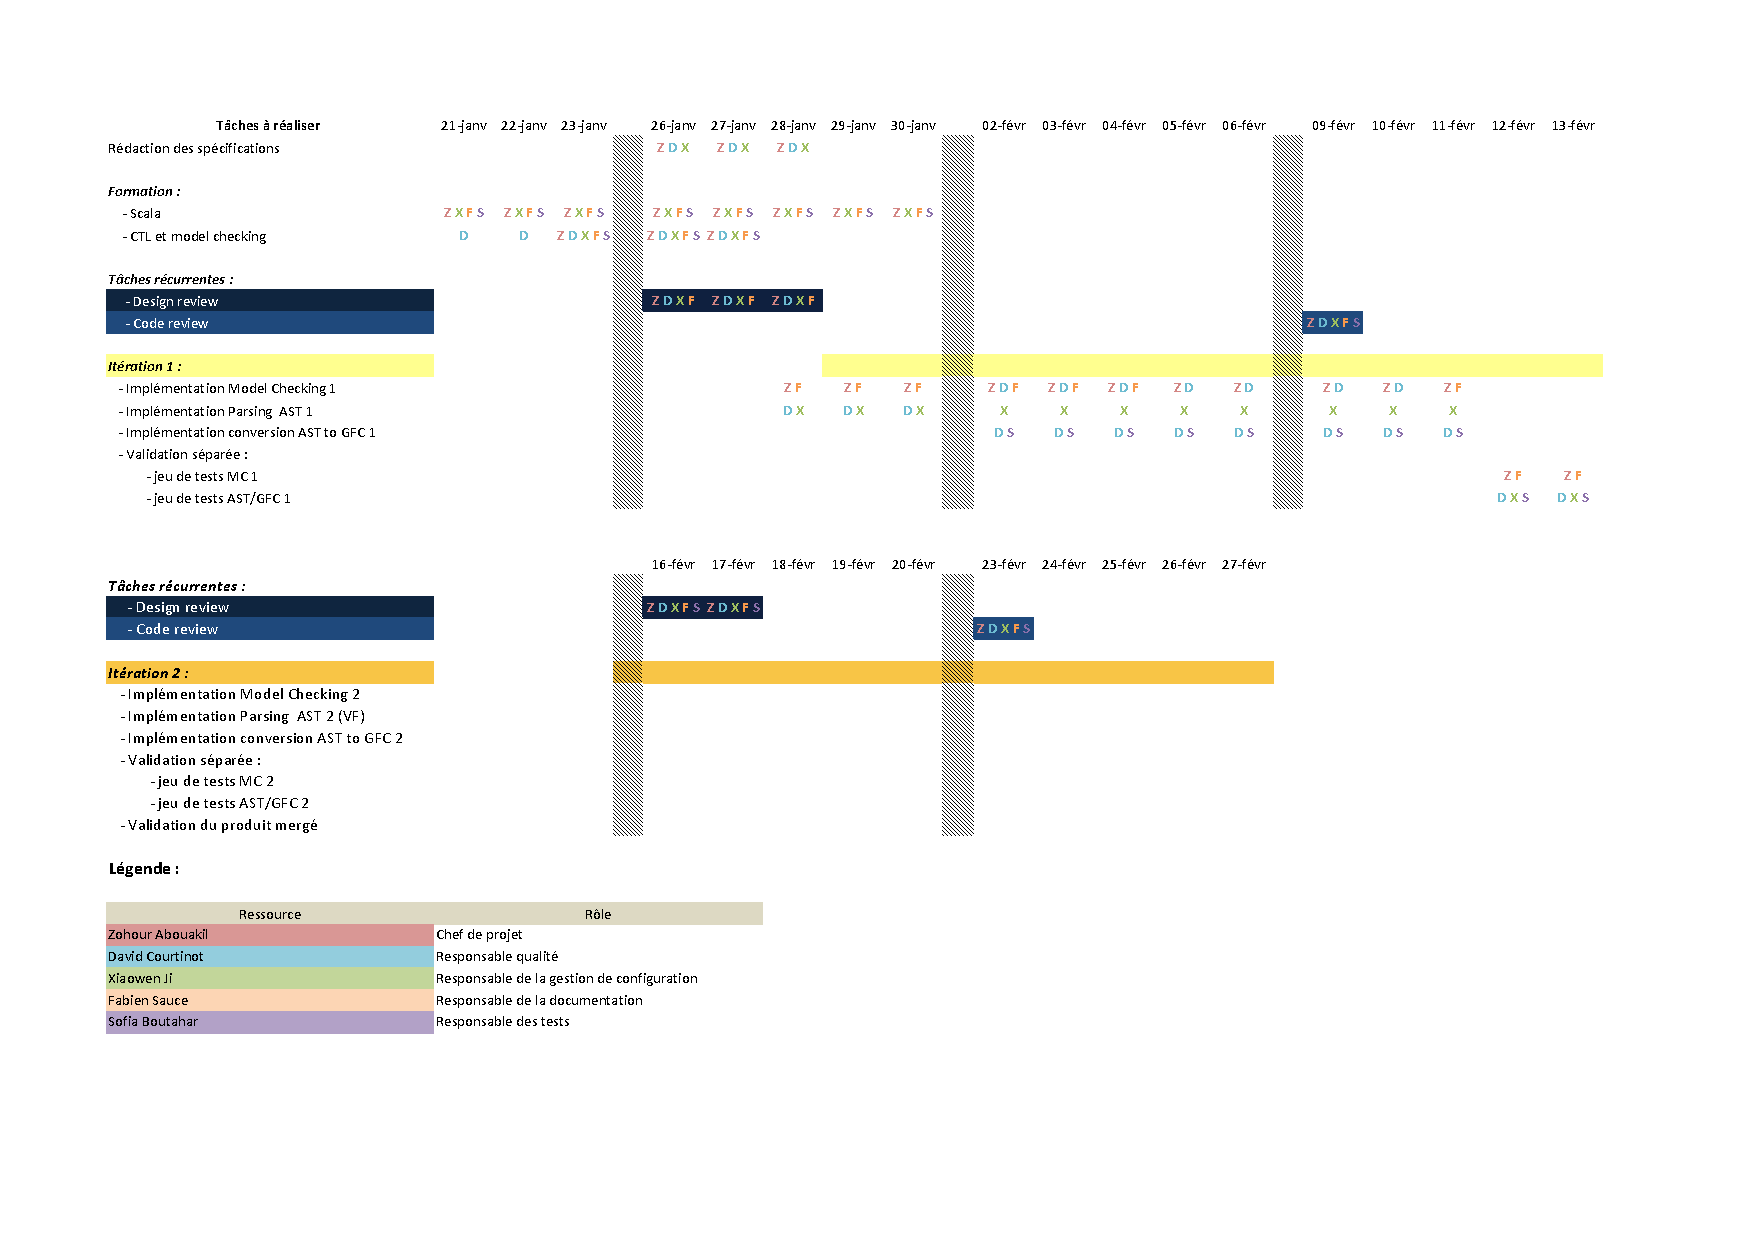
\includepdf[landscape=true,pages={1-2}]{data/planning.pdf}
\chapter{Risk management}

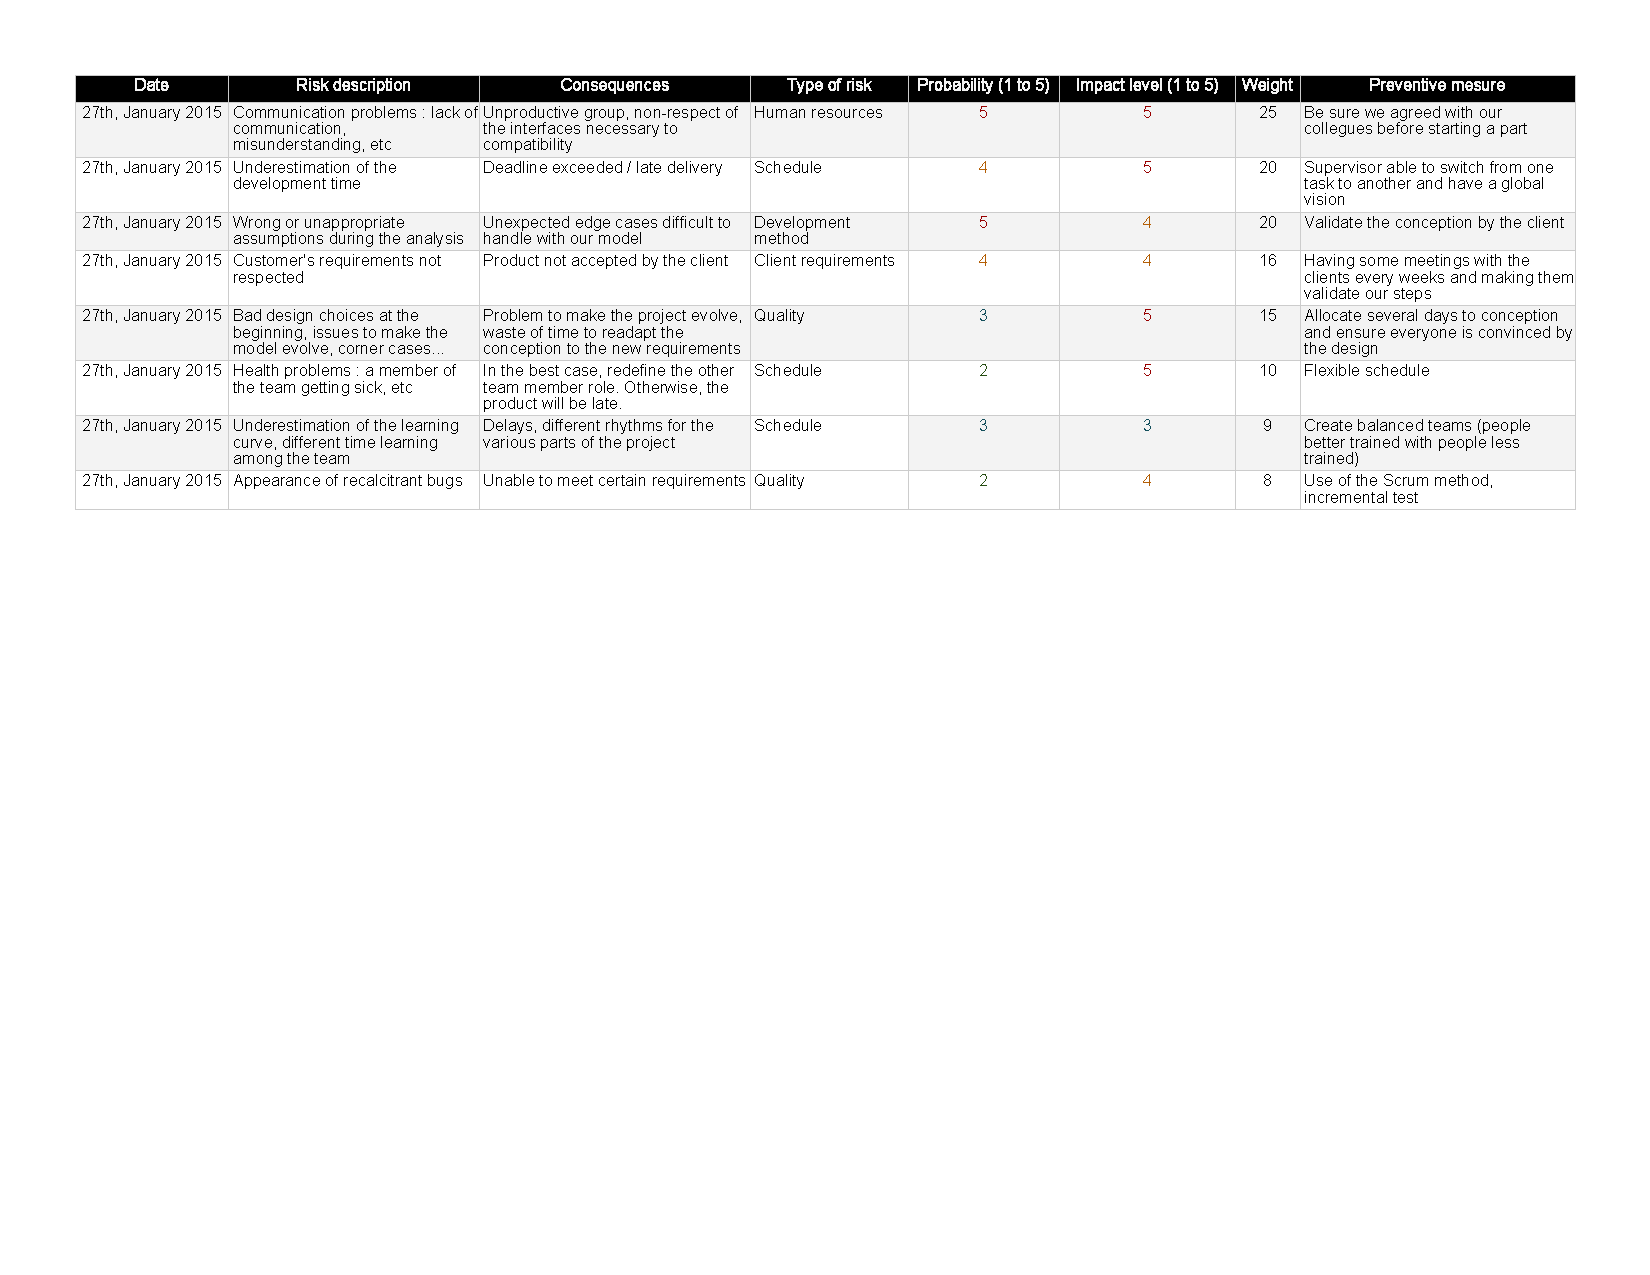
\includepdf[landscape=true,pages={1}]{data/risks.pdf}
\chapter{Code management}

\section{Quality management}

\subsection{Automated coding style checks}

\paragraph{}
\hspace{4mm}\textnormal{For ensuring that our coding rules are respected and evaluate the quality of our sources, we have
used a tool called \textit{Scalastyle} that enables, using an easy-to-use xml configuration file, to check
some properties on a Scala code. Combined with a specific pulgin, this can be use to generate warnings or errors
in the IDE the developer is using. Our settings can be found in appendix A.}

\section{Test strategy}

\paragraph{}
\hspace{4mm}\textnormal{}

\section{Configuration management}

\paragraph{}
\hspace{4mm}\textnormal{}

\chapter{Appendices}

\end{document}
